% Chinese support

\documentclass[a4paper,twoside]{ctexart}
\usepackage{blindtext}  
\usepackage{geometry}


\ctexset{
	section={
		format+ = \zihao{-3} \heiti \raggedright,
		number = \chinese{section}
	}
}

% Page margin layout
\geometry{left=2.3cm,right=2cm,top=2.5cm,bottom=2.0cm}


\usepackage{listings}
\usepackage{xcolor}
\usepackage{geometry}
\usepackage{amsmath}
\usepackage{float}
\usepackage{hyperref}

\usepackage{graphics}
\usepackage{graphicx}
\usepackage{subfigure}
\usepackage{epsfig}
\usepackage{float}

\usepackage{circuitikz}
\usepackage{pbox}
\usepackage{bbding}
\usepackage{karnaugh-map}
\newcommand{\ctikzlabel}[2]{\pbox{\textwidth}{#1\\#2}}


\usepackage{algorithm}
\usepackage[noend]{algpseudocode}

\usepackage{booktabs}
\usepackage{threeparttable}
\usepackage{longtable}
\usepackage{listings}
\usepackage{tikz}
\usepackage{multicol}

% cite package, to clean up citations in the main text. Do not remove.
\usepackage{cite}

\usepackage{color,xcolor}

%% The amssymb package provides various useful mathematical symbols
\usepackage{amssymb}
%% The amsthm package provides extended theorem environments
\usepackage{amsthm}
\usepackage{amsfonts}
\usepackage{enumerate}
\usepackage{enumitem}
\usepackage{listings}

\usepackage{pdfpages}

\usepackage{indentfirst}
\setlength{\parindent}{2em} % Make two letter space in the first paragraph
\usepackage{setspace}
\linespread{1.5} % Line spacing setting
\usepackage{siunitx}
\setlength{\parskip}{0.5em} % Paragraph spacing setting

% \usepackage[contents =22920202204622, scale = 10, color = black, angle = 50, opacity = .10]{background}

\renewcommand{\figurename}{图}
\renewcommand{\lstlistingname}{代码} 
\renewcommand{\tablename}{表格}
\renewcommand{\contentsname}{目录}
\floatname{algorithm}{算法}

\graphicspath{ {images/} }

%%%%%%%%%%%%%
\newcommand{\StudentNumber}{22920202204622}  % Fill your student number here
\newcommand{\StudentName}{熊恪峥}  % Replace your name here
\newcommand{\PaperTitle}{数字逻辑实验(九)}  % Change your paper title here
\newcommand{\PaperType}{实验报告} % Replace the type of your report here
\newcommand{\Date}{2022年6月20日}
\newcommand{\College}{信息学院}
\newcommand{\CourseName}{数字逻辑}
%%%%%%%%%%%%%

%% Page header and footer setting
\usepackage{fancyhdr}
\usepackage{lastpage}
\pagestyle{fancy}
\fancyhf{}
% This requires the document to be twoside
\fancyhead[LO]{\texttt{\StudentName }}
\fancyhead[LE]{\texttt{\StudentNumber}}
\fancyhead[C]{\texttt{\PaperTitle }}
\fancyhead[R]{\texttt{第{\thepage}页,共\pageref*{LastPage}页}}


\title{\PaperTitle}
\author{\StudentName}
\date{\Date}

\lstset{
	basicstyle          =   \sffamily,          % 基本代码风格
	keywordstyle        =   \bfseries,          % 关键字风格
	commentstyle        =   \rmfamily\itshape,  % 注释的风格,斜体
	stringstyle         =   \ttfamily,  % 字符串风格
	flexiblecolumns,                % 别问为什么,加上这个
	numbers             =   left,   % 行号的位置在左边
	showspaces          =   false,  % 是否显示空格,显示了有点乱,所以不现实了
	numberstyle         =   \zihao{-5}\ttfamily,    % 行号的样式,小五号,tt等宽字体
	showstringspaces    =   false,
	captionpos          =   t,      % 这段代码的名字所呈现的位置,t指的是top上面
	frame               =   lrtb,   % 显示边框
}

\lstdefinestyle{PythonStyle}{
	language        =   Python, % 语言选Python
	basicstyle      =   \zihao{-5}\ttfamily,
	numberstyle     =   \zihao{-5}\ttfamily,
	keywordstyle    =   \color{blue},
	keywordstyle    =   [2] \color{teal},
	stringstyle     =   \color{magenta},
	commentstyle    =   \color{red}\ttfamily,
	breaklines      =   true,   % 自动换行,建议不要写太长的行
	columns         =   fixed,  % 如果不加这一句,字间距就不固定,很丑,必须加
	basewidth       =   0.5em,
}

\algnewcommand\algorithmicinput{\textbf{Input:}}
\algnewcommand\algorithmicoutput{\textbf{Output:}}
\algnewcommand\Input{\item[\algorithmicinput]}%
\algnewcommand\Output{\item[\algorithmicoutput]}%

\usetikzlibrary{positioning, shapes.geometric}

\newcommand{\ols}[1]{\mskip.5\thinmuskip\overline{\mskip-.5\thinmuskip {#1} \mskip-.5\thinmuskip}\mskip.5\thinmuskip}

% \usepackage{draftwatermark}
% \SetWatermarkText{22920202204622}
% \SetWatermarkScale{0.8}

\begin{document}
	
%%%%%%%%%%%%%%%%%%%%%%%%%%%%%%%%%%%%%%%%%%%%
\makeatletter % change default title style
\renewcommand*\maketitle{%
	\begin{center} 
		\bfseries  % title 
		{\LARGE \@title \par}  % LARGE typesetting
		\vskip 1em  %  margin 1em
		{\global\let\author\@empty}  % no author information
		{\global\let\date\@empty}  % no date
		\thispagestyle{empty}   %  empty page style
	\end{center}%
	\setcounter{footnote}{0}%
}
\makeatother
%%%%%%%%%%%%%%%%%%%%%%%%%%%%%%%%%%%%%%%%%%%%
	
	
\thispagestyle{empty}

\vspace*{1cm}

\begin{figure}[h]
	\centering
	
\includegraphics[width=4.0cm]{logo.png}
\end{figure}

\vspace*{1cm}

\begin{center}
	\Huge{\textbf{\PaperType}}
	
	\Large{\PaperTitle}
\end{center}

\vspace*{1cm}

\begin{table}[h]
	\centering	
	\begin{Large}
		\renewcommand{\arraystretch}{1.5}
		\begin{tabular}{p{3cm} p{5cm}<{\centering}}
			姓\qquad 名 & \StudentName  \\
			\hline
			学\qquad号 & \StudentNumber \\
			\hline
			日\qquad期 & \Date  \\
			\hline
			学\qquad院 & \College  \\
			\hline
			课程名称 & \CourseName  \\
			\hline
		\end{tabular}
	\end{Large}
\end{table}

\newpage

\title{
	\Large{\textcolor{black}{\PaperTitle}}
}
 
\newpage
\setcounter{page}{1}

\begin{spacing}{1.2}


\includepdf[pages={21,22}]{../instruction.pdf}
\setcounter{section}{6}

\section{实验结果}

\subsection{多谐振荡器}

使用Multisim软件模拟该电路,可以得到波形如图~\ref{fig:91}

\begin{figure}[htbp]
	\centering
	\caption{图9.1波形}
	\label{fig:91}
	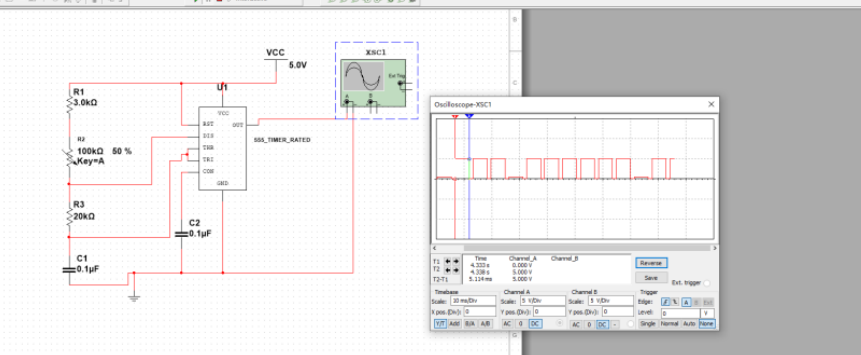
\includegraphics[width=0.64\textwidth]{1.png}
\end{figure}

将电阻调至$7.5k\Omega$,可以发现波形如图~\ref{fig:91b}

\begin{figure}[htbp]
	\centering
	\caption{图9.1波形}
	\label{fig:91b}
	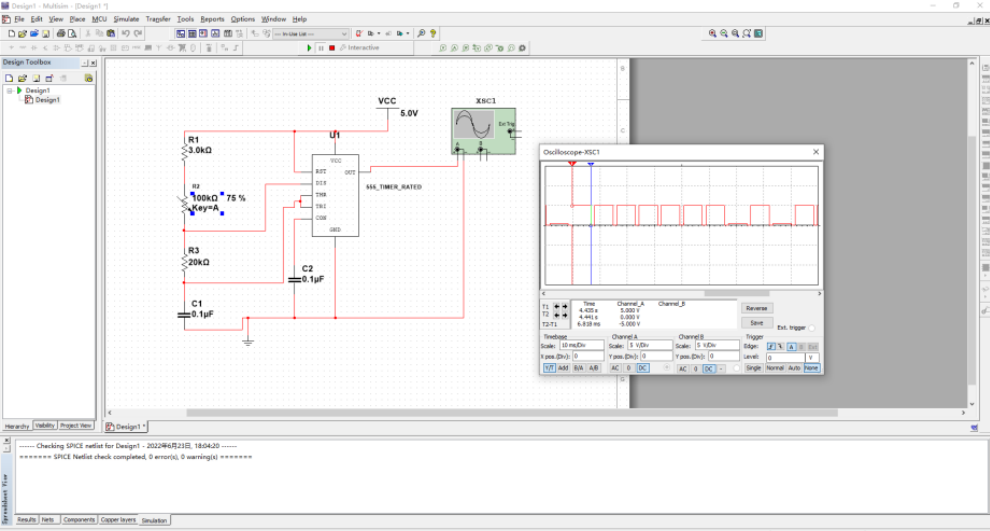
\includegraphics[width=0.64\textwidth]{2.png}
\end{figure}

\subsection{TTL单稳态电路}

模拟TTL与非门单稳态电路的参数,效果如图~\ref{fig:ttl}。

\begin{figure}[htbp]
	\centering
	\caption{TTL与非门单稳态电路}
	\label{fig:ttl}
	\subfigure[$V_{o1}$]{
		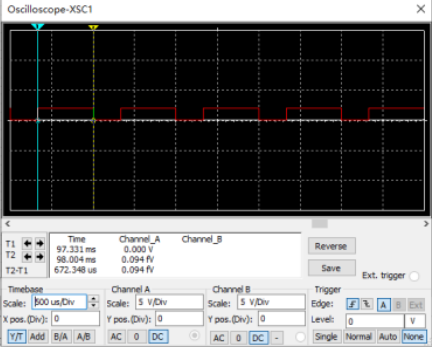
\includegraphics[width=0.48\textwidth]{4a.png}
	}
	\subfigure[$V_{I2}$]{
		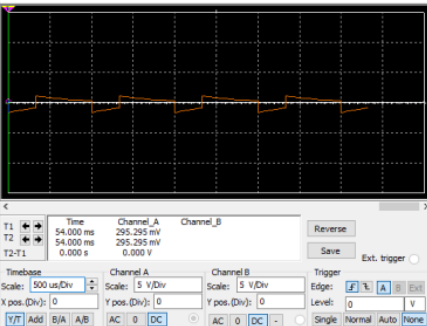
\includegraphics[width=0.48\textwidth]{4b.png}
	}
	\subfigure[$V_{o}$]{
		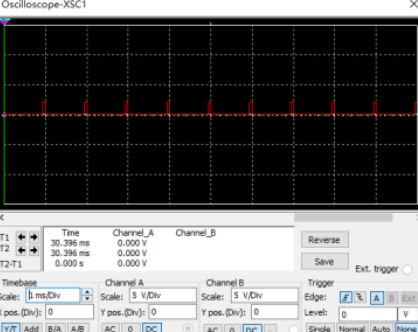
\includegraphics[width=0.48\textwidth]{4c.png}
	}
\end{figure}

\subsection{555定时器单稳态电路}

模拟555定时器单稳态电路的参数,效果如图~\ref{fig:555}。

\begin{figure}[htbp]
	\centering
	\caption{TTL与非门单稳态电路}
	\label{fig:555}
	\subfigure[$V_{I}$]{
		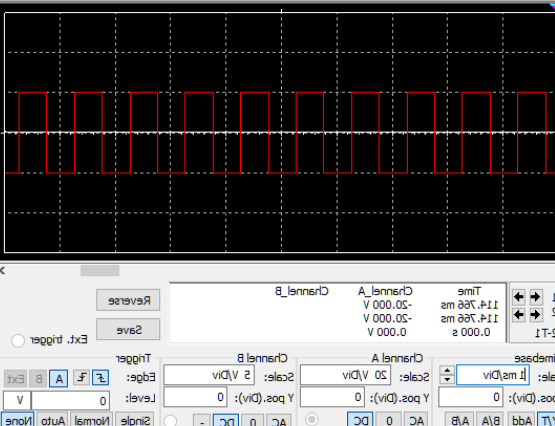
\includegraphics[width=0.48\textwidth]{5.png}
	}
	\subfigure[$V_{C}$]{
		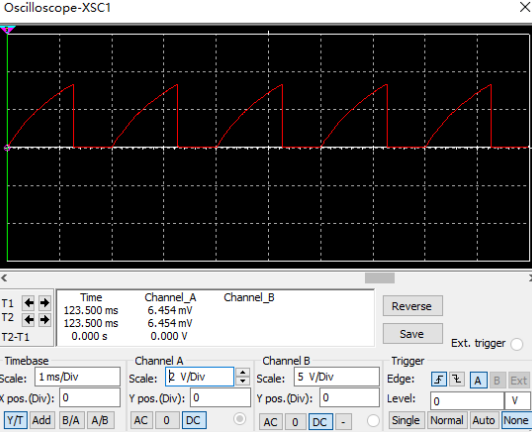
\includegraphics[width=0.48\textwidth]{6.png}
	}
	\subfigure[$V_{O}$]{
		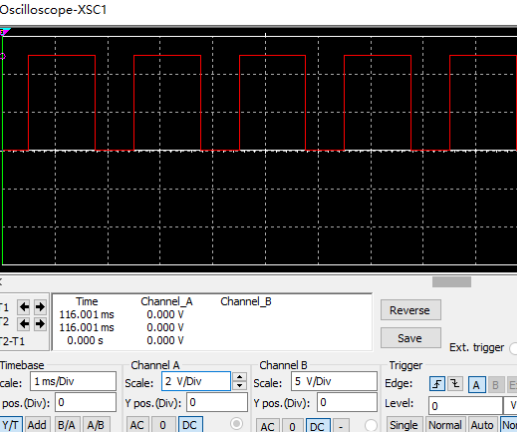
\includegraphics[width=0.48\textwidth]{7.png}
	}
\end{figure}

\section{实验总结}

通过本次实验,我练习了使用软件模拟电路的方法。软件模拟是一种方便快捷
有效的学习数字电路、设计数字电路的方法。

\end{spacing}

\end{document}